% F091｜完全立方数的立方根尾数速判｜05_traps.tex
% 继承上传模板的 LaTeX 环境；当前条目的内容独立编写。
\clearpage
\begin{trapbox}
\textbf{\textcolor{CTrap}{易错一：未保证完全立方就直接报整数根}}
\par\medskip
\begin{center}
% F091｜verify 原创简明教学示意图
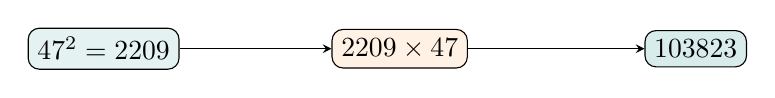
\begin{tikzpicture}[>=stealth,scale=.94]
\node[draw,fill=teal!10,rounded corners] (a) at (0,0){$47^2=2209$};
\node[draw,fill=orange!10,rounded corners] (b) at (4,0){$2209\times47$};
\node[draw,fill=teal!15,rounded corners] (c) at (8,0){$103823$};
\draw[->] (a)--(b);\draw[->] (b)--(c);
\end{tikzpicture}

\end{center}
\medskip
例如 $\sqrt[3]{103824}$ 不是整数 $47$；尾数模式只用于已知是\textbf{完全立方数}的情形，不能将近似结果误当精确值。
\end{trapbox}
\clearpage
\begin{trapbox}
\textbf{\textcolor{CTrap}{易错二：高位分组位置搞错}}
\par\medskip
\begin{center}
% F091｜split 原创简明教学示意图
\begin{tikzpicture}[>=stealth,scale=.9]
\node[draw,rounded corners,fill=teal!9,minimum width=2.5cm,minimum height=1.25cm] (a) at (0,0){$\underbrace{103}_{\text{高位}}\mid\underbrace{823}_{\text{低位}}$};
\node[draw,rounded corners,fill=orange!9,minimum width=3.2cm,minimum height=1.25cm] (b) at (4.5,0){$4^3\le103<5^3$};
\node[draw,rounded corners,fill=teal!15,minimum width=2.3cm,minimum height=1.25cm] (c) at (9.0,0){$\sqrt[3]{103823}=47$};
\draw[->,thick] (a)--(b);\draw[->,thick] (b)--(c);
\node at (4.5,-1.2){\small 高位定十位，末位定个位};
\end{tikzpicture}

\end{center}
\medskip
应按\textbf{从右往左每三位}分组，$103823$ 写作 $103\mid823$，而不是 $10\mid3823$。
\end{trapbox}
\clearpage
\begin{trapbox}
\textbf{\textcolor{CTrap}{易错三：把立方数末位当根的末位}}
\par\medskip
\begin{center}
% F091｜table 原创简明教学示意图
\begin{tikzpicture}[>=stealth,scale=.94]
\node[draw,rounded corners,fill=teal!10,align=center,minimum width=9.4cm,minimum height=1.1cm] at (4,0){$0\!\to\!0,\ 1\!\to\!1,\ 2\!\to\!8,\ 3\!\to\!7,\ 4\!\to\!4$\\$5\!\to\!5,\ 6\!\to\!6,\ 7\!\to\!3,\ 8\!\to\!2,\ 9\!\to\!9$};
\node at (4,-1.15){\small 箭头表示“某个位数立方后的个位”};
\end{tikzpicture}

\end{center}
\medskip
末位 $8$ 的立方数，其整数根末位是 $2$（$2^3=8$）；末位 $2$ 的立方数，其根末位是 $8$（$8^3=512$）。
\end{trapbox}
